\documentclass[11pt,a4paper]{article}
\usepackage{lmodern}


\usepackage{amssymb,amsmath}
\usepackage{ifxetex,ifluatex}
\usepackage{fixltx2e} % provides \textsubscript
\ifnum 0\ifxetex 1\fi\ifluatex 1\fi=0 % if pdftex
  \usepackage[T1]{fontenc}
  \usepackage[utf8]{inputenc}
\else % if luatex or xelatex
  \ifxetex
    \usepackage{mathspec}
    \usepackage{xltxtra,xunicode}
  \else
    \usepackage{fontspec}
  \fi
  \defaultfontfeatures{Mapping=tex-text,Scale=MatchLowercase}
  \newcommand{\euro}{€}
\fi
% use upquote if available, for straight quotes in verbatim environments
\IfFileExists{upquote.sty}{\usepackage{upquote}}{}
% use microtype if available

\usepackage[lmargin=5cm,rmargin=2.5cm,tmargin=2.5cm,bmargin=2.5cm]{geometry}

% Figure Placement:
\usepackage{float}
\let\origfigure\figure
\let\endorigfigure\endfigure
\renewenvironment{figure}[1][2] {
    \expandafter\origfigure\expandafter[H]
} {
    \endorigfigure
}

%% citation setup

\usepackage{csquotes}

\usepackage[backend=biber, maxbibnames = 99, style = apa]{biblatex}
\setlength\bibitemsep{1.5\itemsep}
\bibliography{Resources/references.bib}
\usepackage{longtable,booktabs}
\usepackage{graphicx}
\makeatletter
\def\maxwidth{\ifdim\Gin@nat@width>\linewidth\linewidth\else\Gin@nat@width\fi}
\def\maxheight{\ifdim\Gin@nat@height>\textheight\textheight\else\Gin@nat@height\fi}
\makeatother
% Scale images if necessary, so that they will not overflow the page
% margins by default, and it is still possible to overwrite the defaults
% using explicit options in \includegraphics[width, height, ...]{}
\setkeys{Gin}{width=\maxwidth,height=\maxheight,keepaspectratio}
\ifxetex
  \usepackage[setpagesize=false, % page size defined by xetex
              unicode=false, % unicode breaks when used with xetex
              xetex]{hyperref}
\else
  \usepackage[unicode=true]{hyperref}
\fi
\hypersetup{breaklinks=true,
            bookmarks=true,
            pdfauthor={Rezaul Hoque, Sarah Al-Talal},
            pdftitle={Predicting Residential Construction Year and Classifying Architectural Typology: A Machine Learning Study on the Ames Housing Dataset},
            colorlinks=true,
            citecolor=blue,
            urlcolor=blue,
            linkcolor=black,
            pdfborder={0 0 0}}
\urlstyle{same}  % don't use monospace font for urls
\setlength{\parindent}{0pt}
\setlength{\parskip}{6pt plus 2pt minus 1pt}
\setlength{\emergencystretch}{3em}  % prevent overfull lines
\setcounter{secnumdepth}{5}

%%% Use protect on footnotes to avoid problems with footnotes in titles
\let\rmarkdownfootnote\footnote%
\def\footnote{\protect\rmarkdownfootnote}

%%% Change title format to be more compact
\usepackage{titling}

% Acronyms package defining
\urlstyle{same}  % don't use monospace font for urls

% Create subtitle command for use in maketitle
\newcommand{\subtitle}[1]{
  \posttitle{
    \begin{center}\large#1\end{center}
    }
}

\setlength{\droptitle}{-2em}
  \title{Predicting Residential Construction Year and Classifying
Architectural Typology: A Machine Learning Study on the Ames Housing
Dataset}
  \pretitle{\vspace{\droptitle}\centering\huge}
  \posttitle{\par}
\subtitle{Statistical Learning}
  \author{Rezaul Hoque, Sarah Al-Talal}
  \preauthor{\centering\large\emph}
  \postauthor{\par}
  \predate{\centering\large\emph}
  \postdate{\par}
  \date{today}

\usepackage{array}
\usepackage{calc}
\providecommand{\real}[1]{#1}
\providecommand{\tightlist}{\setlength{\itemsep}{0pt}\setlength{\parskip}{0pt}}
\let\oldsection\section
\renewcommand{\section}{\clearpage\oldsection}

%% linespread settings

\usepackage{setspace}

\onehalfspacing

% Language Setup

\usepackage{ifthen}
\usepackage{iflang}
\usepackage[super]{nth}

\ifthenelse{\equal{english}{german}}{
  \usepackage[ngerman]{babel}
  }{
  \usepackage[english]{babel}
  }

\IfFileExists{microtype.sty}{%
	\usepackage[nopatch=footnote]{microtype}
	\UseMicrotypeSet[protrusion]{basicmath} % disable protrusion for tt fonts
}{}
%\makeatletter
%\providecommand{\pandocbounded}[1]{%
%  \begin{minipage}[t]{\linewidth}%
%    \def\maxwidth{\linewidth}%
%    \def\maxheight{\textheight}%
%    \setkeys{Gin}{width=\maxwidth,height=\maxheight,keepaspectratio}%
%    #1%
%  \end{minipage}%
%}
%\makeatother

% escape pandocbounded
\newcommand{\pandocbounded}[1]{#1}

\begin{document}

\newgeometry{left=2cm,right=1cm,bottom=2cm,top=2cm}

\begin{titlepage}
  \noindent\begin{minipage}{0.6\textwidth}
	  \IfLanguageName{english}{University of Duisburg-Essen}{Universität Duisburg-Essen}\\
	  \IfLanguageName{english}{Faculty of Business Administration and Economics}{Fakultät für Wirtschaftswissensschaften}\\
	  \IfLanguageName{english}{Chair of Econometrics}{Lehrstuhl für Ökonometrie}\\
  \end{minipage}
	\begin{minipage}{0.4\textwidth}
	  \begin{flushright}
  	  \vspace{-0.5cm}
      \IfLanguageName{english}{\includegraphics*[width=5cm]{Resources/duelogo_en.png}}{\includegraphics*[width=5cm]{Resources/duelogo_de.png}}
	  \end{flushright}
	\end{minipage}
  \\
  \vspace{1.5cm}
  \begin{center}
  \huge{Predicting Residential Construction Year and Classifying
Architectural Typology: A Machine Learning Study on the Ames Housing
Dataset}\\
  \vspace{.25cm}
  \Large{Statistical Learning}\\
  \vspace{0.5cm}
  \large{Term Paper}\\
  \vspace{1cm}
  \large{
  \IfLanguageName{english}{Submitted to the Faculty of \\ Business Administration and Economics \\at the \\University of Duisburg-Essen}{Vorgelegt der \\Fakultät für Wirtschaftswissenschaften der \\ Universität Duisburg-Essen}\\}
  \vspace{0.75cm}
  \large{\IfLanguageName{english}{from:}{von:}}\\
  \vspace{0.5cm}
  Rezaul Hoque, Sarah Al-Talal\\
  \end{center}
  \vspace{4cm}
  
 
  

  \noindent\begin{minipage}[t]{0.5\textwidth}
  \IfLanguageName{english}{Matriculation Number:}{Matrikelnummer}
  \end{minipage}
  \begin{minipage}[t]{0.7\textwidth}
  \hspace{1cm}Your Matriculation Number
  \end{minipage}

  \noindent\begin{minipage}[t]{0.5\textwidth}
  \IfLanguageName{english}{Study Path:}{Studienfach:}
  \end{minipage}
  \begin{minipage}[t]{0.7\textwidth}
  \hspace{1cm}Information Systems
  \end{minipage}

  \noindent\begin{minipage}[t]{0.5\textwidth}
  \IfLanguageName{english}{Reviewer:}{Erstgutachter:}
  \end{minipage}
  \begin{minipage}[t]{0.7\textwidth}
  \hspace{1cm}
  \end{minipage}

  \noindent\begin{minipage}[t]{0.5\textwidth}
  \IfLanguageName{english}{Secondary Reviewer:}{Zweitgutachter}
  \end{minipage}
  \begin{minipage}[t]{0.7\textwidth}
  \hspace{1cm}
  \end{minipage}

  \noindent\begin{minipage}[t]{0.5\textwidth}
  Semester:
  \end{minipage}
  \begin{minipage}[t]{0.7\textwidth}
  \hspace{1cm}\IfLanguageName{english}{\nth{1} Semester}{1. Fachsemester}
  \end{minipage}

  \noindent\begin{minipage}[t]{0.5\textwidth}
  \IfLanguageName{english}{Graduation (est.):}{Vsl. Studienabschluss:}
  \end{minipage}
  \begin{minipage}[t]{0.7\textwidth}
  \hspace{1cm}Summer Term 2026
  \end{minipage}

  \noindent\begin{minipage}[t]{0.5\textwidth}
  \IfLanguageName{english}{Deadline:}{Abgabefrist:}
  \end{minipage}
  \begin{minipage}[t]{0.7\textwidth}
  \hspace{1cm}July 17, 2026
  \end{minipage}

\end{titlepage}


% Ends the declared geometry for the titlepage
\restoregeometry

\begin{abstract}
This paper applies supervised machine learning to the Ames Housing
Dataset to address two prediction tasks that are independent of market
valuation. The first task is a regression problem: estimating a
residential property's original construction year from its physical
attributes and quality ratings. The second is a four-class
classification problem: predicting a property's architectural typology
from its spatial and structural measurements. Nine regression models and
eight classification models were trained within a leakage-safe
preprocessing pipeline, evaluated on a held-out test set, and the four
best-performing models per task were further refined through
hyperparameter tuning. Random Forest achieved the strongest regression
performance using its default hyperparameters (RMSE of 4.85 years,
R\textsuperscript{2} = 0.973), while tuned XGBoost achieved the
strongest classification performance (macro-averaged F1 score of 0.837
and an accuracy of 91.8\%). The results demonstrate that physical design
attributes encode a recoverable signal about both construction era and
structural form, and that tree-based ensemble methods are the most
effective strategy for recovering it from tabular housing data.
\end{abstract}
\newpage

\pagenumbering{Roman} 
{
\hypersetup{linkcolor=black}
\setcounter{tocdepth}{3}
\tableofcontents
}



\newpage
\listoftables
\newpage
\listoffigures
\newpage
\pagenumbering{arabic} 
\section{Introduction}\label{introduction}

The Ames Housing Dataset \autocite{DeCock2011} documents 2,930
residential property sales in Ames, Iowa between 2006 and 2010 and
contains 82 variables covering physical dimensions, material quality
ratings, basement and garage attributes, and neighbourhood
classification. While the dataset is most commonly applied to predicting
sale price, this study redirects attention to the structural and
architectural information embedded in the physical record of each
property.

While much of the existing literature applies machine learning to
residential property price prediction
\autocite{ChoyHo2023,HoTangWong2020,JinXu2025}, previous studies have
extensively applied the dataset to residential property price prediction
while also identifying the housing characteristics that most strongly
influence market value \autocite{HoTangWong2020,TeohEtAl2023}.

Two prediction tasks motivate the analysis. The first is a regression
problem: estimating the original year of construction from a property's
physical attributes and quality ratings, without access to temporal
metadata or market data. The hypothesis is that construction era leaves
a measurable signature in material choices, room configurations, and the
presence of amenities that changed systematically across the twentieth
century. The second task is a four-class classification problem:
predicting a property's architectural typology --- whether it is
single-story, multi-story, one-and-a-half story, or split-level --- from
its spatial and structural measurements. The goal here is to establish
which geometric features most reliably distinguish residential forms.

By shifting the prediction targets while using the same rich set of
structural, spatial and qualitative housing characteristics, this
project demonstrates an alternative application of the Ames Housing
dataset.

Both tasks are treated as independent prediction problems sharing a
common preprocessing pipeline. Nine regression algorithms and eight
classification algorithms are compared, selected to represent a range of
learning strategies from interpretable linear models to opaque ensemble
methods. A key concern throughout is not only predictive performance but
also the degree to which each model class supports interpretation of its
results.

\section{Exploratory Data Analysis}\label{exploratory-data-analysis}

The Ames Housing dataset used in this project contains 2,930 residential
property observations described by 82 variables, excluding the unique
identifier. These variables capture a broad range of structural,
spatial, and qualitative characteristics of residential properties sold
in Ames, Iowa. The diversity of the available features provides a
comprehensive representation of each property, making the dataset well
suited for supervised machine learning applications.

The dataset consists of both numerical and categorical variables.
Numerical variables describe measurable characteristics such as lot
area, above-ground living area, garage capacity, construction year and
basement size. Categorical variables capture qualitative information
including neighborhood, building type, exterior materials, heating
quality, roof style, and kitchen quality. The combination of numerical
and categorical attributes enables machine learning models to learn
complex relationships between different aspects of residential
properties.

For this project, the dataset is used to address two supervised learning
tasks. The regression task predicts a property construction year
(\texttt{Year\ Built}), while the classification task predicts its
architectural style (\texttt{House\ Style}). All remaining relevant
variables serve as predictor variables after the preprocessing
procedures described in Chapter 3.

Table 1 provides an overview of the dataset characteristics before
preprocessing.

\begin{longtable}[]{@{}ll@{}}
\caption{Dataset
Characteristics.}\label{tbl-dataset-characteristics}\tabularnewline
\toprule\noalign{}
Characteristics & Value \\
\midrule\noalign{}
\endfirsthead
\toprule\noalign{}
Characteristics & Value \\
\midrule\noalign{}
\endhead
\bottomrule\noalign{}
\endlastfoot
Dataset & Ames Housing Dataset \\
Source & Kaggle \\
Observations & 2,930 \\
Variables & 82 \\
Numerical Variables & 39 \\
Categorical Variables & 43 \\
Regression Target & Year Built \\
Classification Target & House Style \\
\end{longtable}

\subsection{Target Variable
Distributions}\label{target-variable-distributions}

\textbf{Year Built.} Construction years span from 1872 to 2010, with a
mean of 1971.4 and a standard deviation of 30.2 years. The distribution
is moderately left-skewed (skewness = \(-0.604\), kurtosis =
\(-0.502\)), reflecting the historical accumulation of housing stock ---
few nineteenth-century properties survive in the sample, while the bulk
of observations are concentrated from the mid-twentieth century onward.
Figure \ref{fig:yearbuilt} illustrates this distribution.

\begin{figure}[htbp]

{\centering 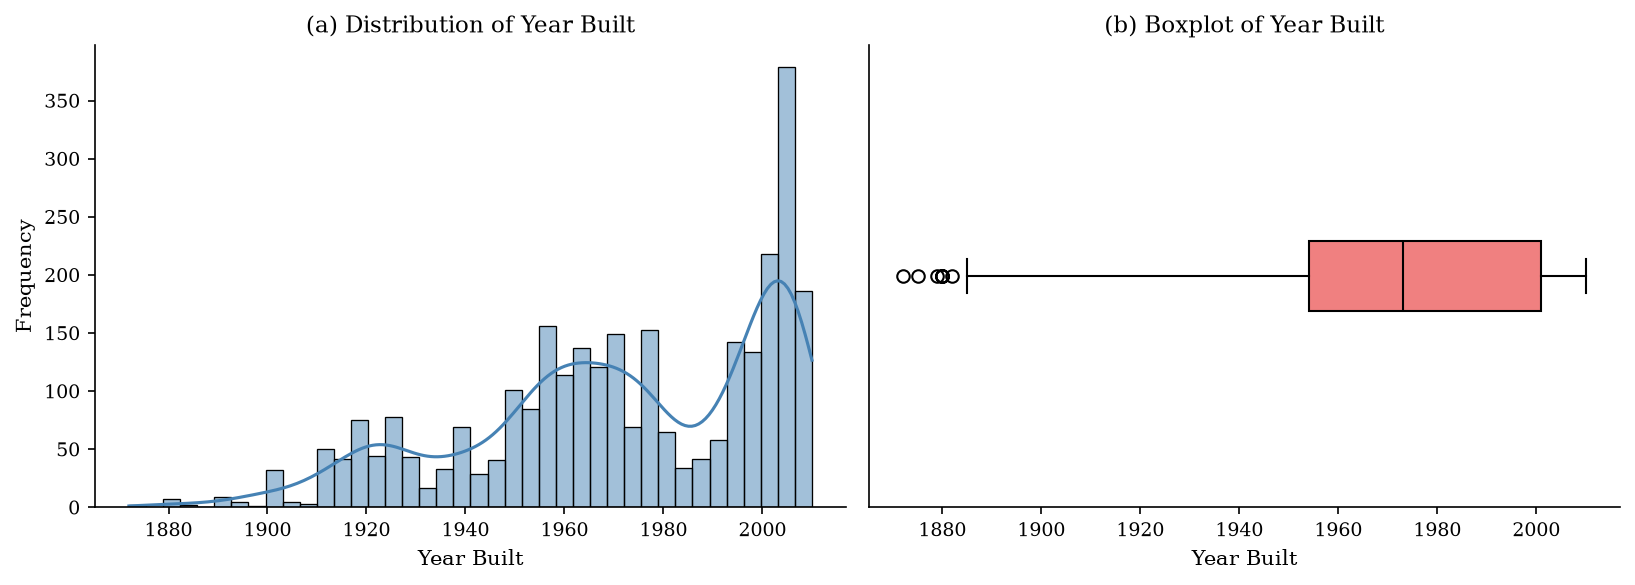
\includegraphics[width=\textwidth]{figures/fig_yearbuilt_dist} 

}

\caption{\label{fig:yearbuilt}Distribution of Year Built: histogram with kernel density estimate (left) and boxplot (right). The left-skewed shape reflects the uneven historical accumulation of housing stock in the dataset.}\label{fig:fig-yearbuilt}
\end{figure}

\textbf{House Style.} The original dataset records eight architectural
style codes. For modelling purposes, these are consolidated into four
typology classes: Single-story (n = 1,481; 50.5\%), Multi-story (n =
905; 30.9\%), 1.5-story (n = 333; 11.4\%), and Split-level (n = 211;
7.2\%). The distribution is considerably imbalanced, with the
Single-story class containing more than twice the observations of the
next largest class. This imbalance has direct implications for the
choice of classification evaluation metric, as discussed in Section
\ref{model-selection}. Figure \ref{fig:housestyle} shows the class
counts before and after consolidation.

\begin{figure}[htbp]

{\centering 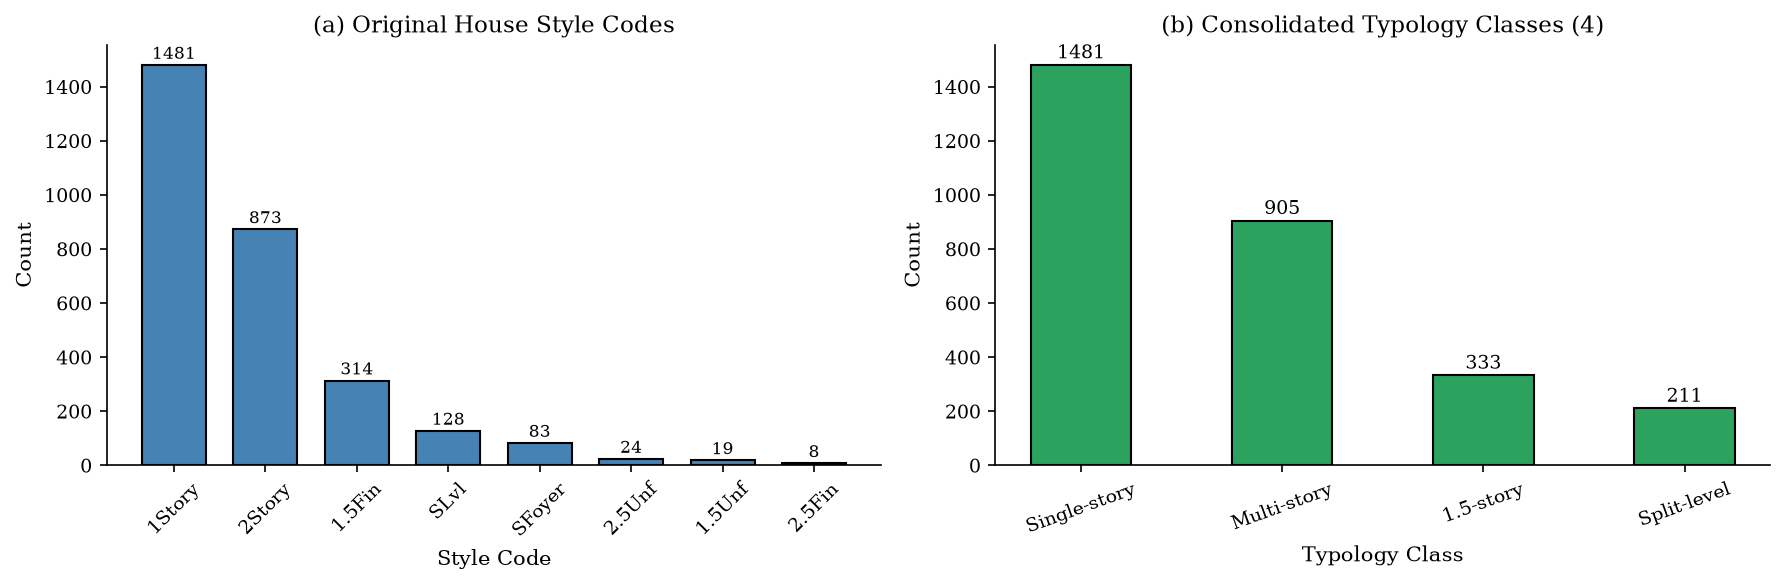
\includegraphics[width=\textwidth]{figures/fig_housestyle_dist} 

}

\caption{\label{fig:housestyle}House Style distribution. Left: the original eight style codes. Right: the four typology classes used in modelling, formed by grouping related codes.}\label{fig:fig-housestyle}
\end{figure}

\subsection{Predictor Relationships}\label{predictor-relationships}

Pearson correlations between numerical predictors and Year Built were
computed to identify features carrying a temporal signal. Figure
\ref{fig:correlation} displays the 12 largest positive and 12 largest
negative correlates. Garage Year Built has the strongest positive
association, reflecting the common practice of constructing the garage
alongside the main dwelling. Overall Quality and Ground Living Area are
also strongly positively correlated, consistent with the historical
trend towards higher-grade materials and larger floor plans in more
recent construction. Negative correlates include variables associated
with older residential conventions, such as Enclosed Porch area and
certain basement configurations.

\begin{figure}[htbp]

{\centering 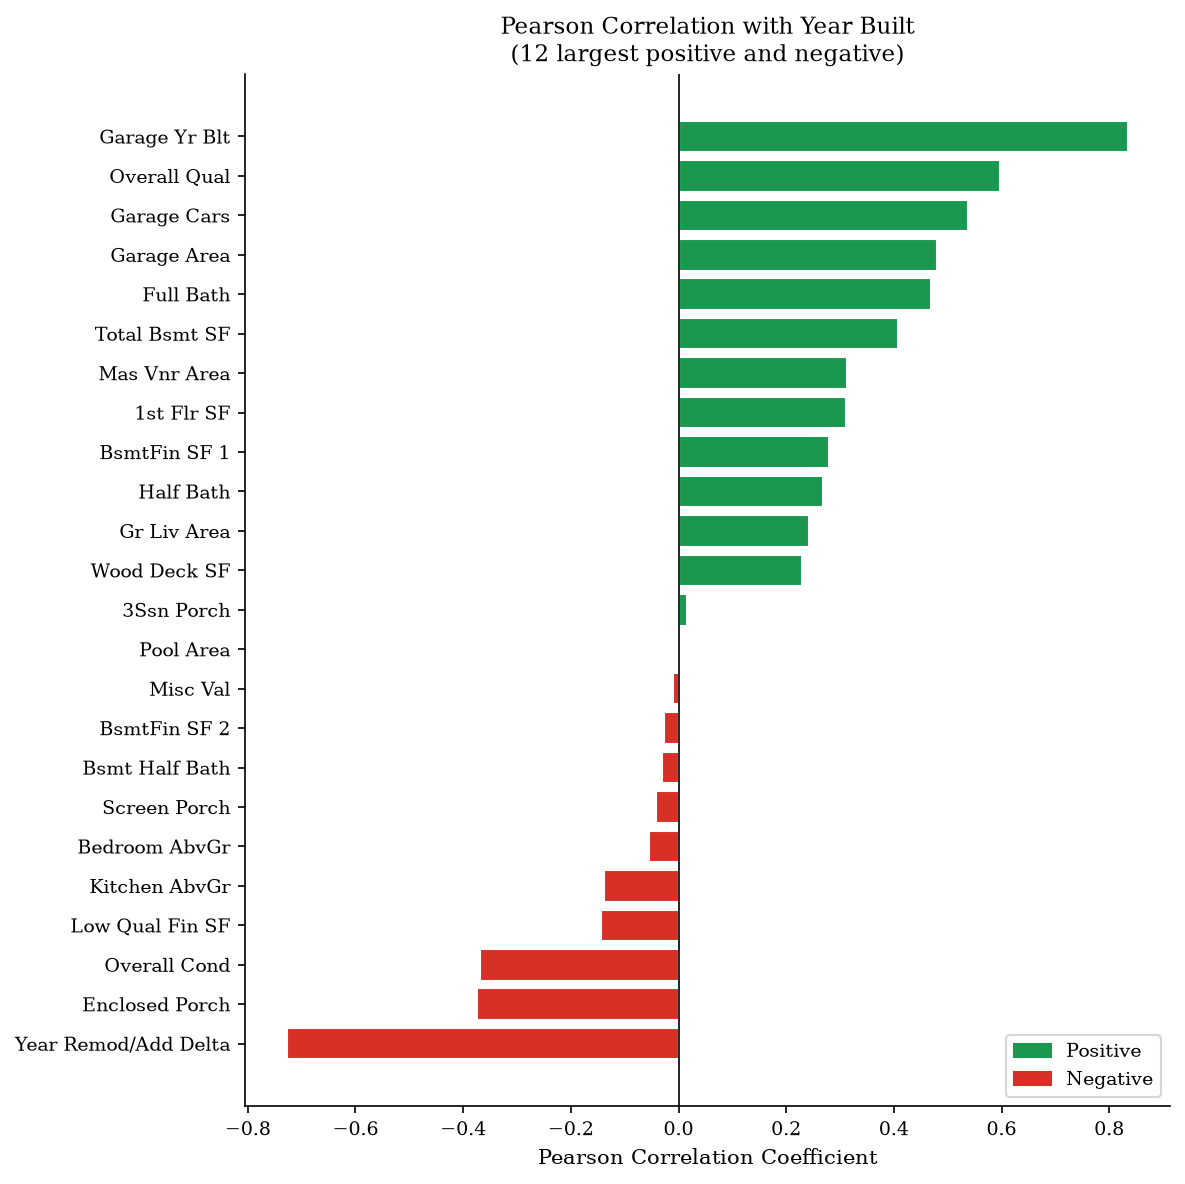
\includegraphics[width=0.85\textwidth]{figures/fig_correlation} 

}

\caption{\label{fig:correlation}Pearson correlation between numerical predictors and Year Built. Green bars indicate positive correlations; red bars indicate negative correlations. The 12 strongest in each direction are shown.}\label{fig:fig-correlation}
\end{figure}

Figure \ref{fig:scatter} confirms these relationships through scatter
plots of the six most strongly correlated predictors. The near-linear
association between Garage Year Built and Year Built is particularly
pronounced. Overall Quality shows a step-pattern consistent with the
periodic revision of building standards. The Year Remod/Add Delta
feature --- the number of years between construction and last remodel
--- is zero for properties that have never been renovated (the
majority), which generates a distinctive clustering near zero.

\begin{figure}[htbp]

{\centering 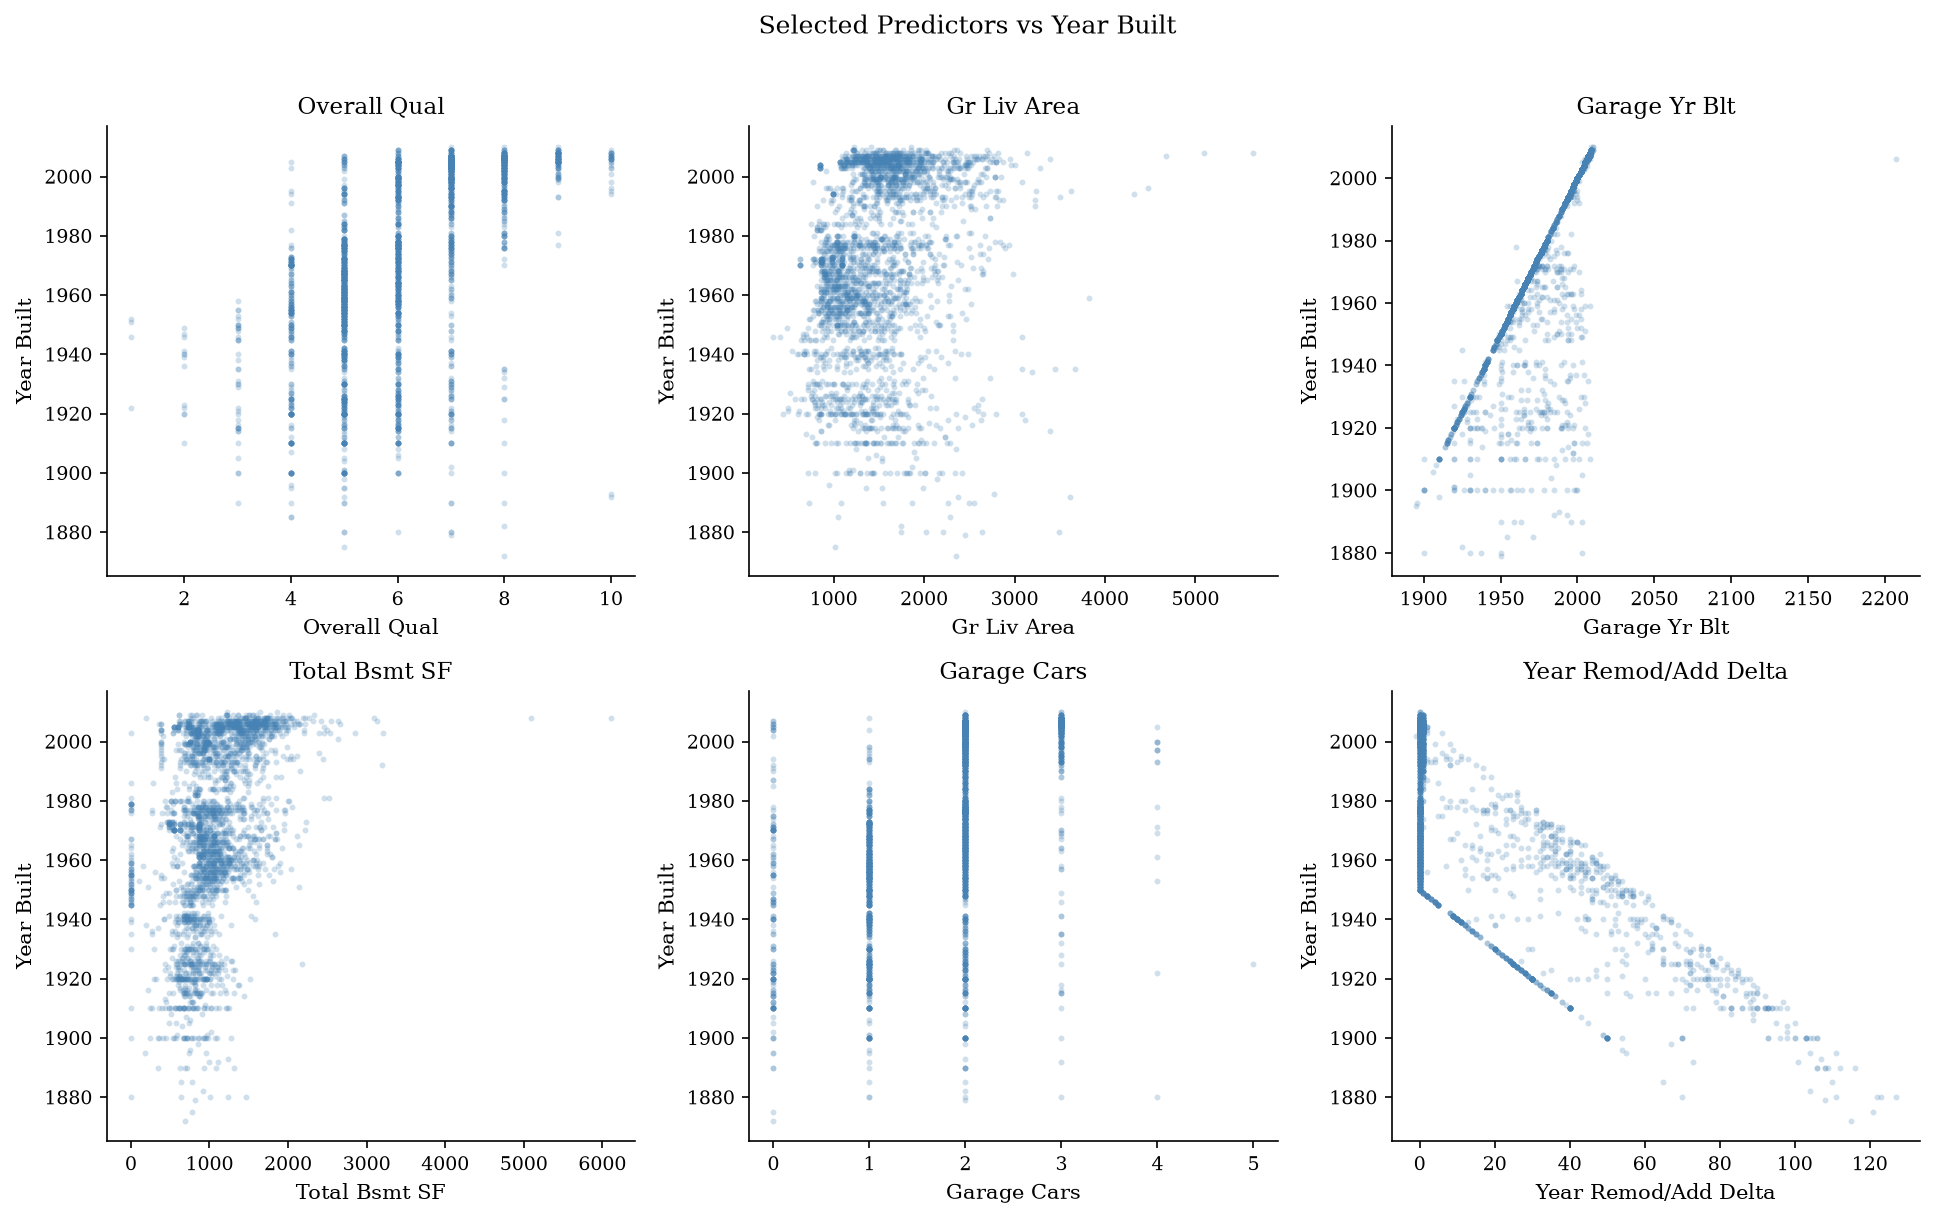
\includegraphics[width=\textwidth]{figures/fig_scatter_predictors} 

}

\caption{\label{fig:scatter}Scatter plots of six key numerical predictors against Year Built. Each point represents one property.}\label{fig:fig-scatter}
\end{figure}

\section{Data Preprocessing}\label{data-preprocessing}

\subsection{Missing Value Handling}\label{missing-value-handling}

Four columns were removed prior to analysis: \texttt{Alley},
\texttt{Pool\ QC}, \texttt{Fence}, and \texttt{Misc\ Feature}, each with
more than 70\% missing values. Imputing columns at this level of
missingness risks distorting the distribution beyond the informative
range of the variable. Following this step, the dataset retained 78
variables. Any rows missing either target variable were subsequently
removed, leaving 2,930 usable observations.

For the remaining missing values, imputation is handled inside the
modelling pipeline rather than on the full dataset. Numerical features
are imputed with the column median; categorical features are imputed
with the mode. Keeping these steps inside the pipeline ensures that
imputation statistics are estimated from the training fold only.

\subsection{Feature Engineering}\label{feature-engineering}

A derived variable, \texttt{Year\ Remod/Add\ Delta}, is computed as the
difference between the recorded remodel year and the construction year.
This captures how recently a property was renovated relative to its
build date without retaining the raw remodel year, which correlates
directly with the regression target. The raw remodel year was then
dropped.

Columns representing administrative identifiers (\texttt{Order},
\texttt{PID}) and sale circumstances (\texttt{SalePrice},
\texttt{Yr\ Sold}, \texttt{Mo\ Sold}) were excluded from both feature
sets. \texttt{House\ Style} is copied to a separate series before being
dropped from the shared feature frame so that it remains available as
the classification target without functioning as a predictor for
regression.

\subsection{Encoding and Scaling}\label{encoding-and-scaling}

Feature types were divided into five groups, each receiving an
appropriate transformation. Sixteen numerical features with
approximately symmetric distributions were assigned to a standardisation
group: a Yeo-Johnson power transform was applied to reduce residual
skew, followed by standardisation to zero mean and unit variance. Eight
features with higher skewness were normalised instead, using the same
power transform followed by min-max scaling. Twenty-one categorical
features with a natural ordering (quality and condition ratings) were
encoded with \texttt{OrdinalEncoder} using explicit category lists.
Nominal features with fewer than ten distinct values received one-hot
encoding, and high-cardinality features received binary encoding to
limit dimensionality expansion.

\subsection{Leakage-Safe Pipeline}\label{leakage-safe-pipeline}

All transformation steps were assembled into a single
\texttt{ColumnTransformer} composed of five sub-pipelines, one per
feature group. The transformer was embedded in a scikit-learn
\texttt{Pipeline} \autocite{Pedregosa2011} alongside each estimator.
This design ensures that imputers, scalers, and encoders are fitted
exclusively on training data. Fitting any of these steps before the
train/test split --- a common but methodologically problematic shortcut
--- would introduce leakage: the imputer would borrow test-set values
into training medians, and the scaler would align training bounds to the
global distribution.

\subsection{Train/Test Split}\label{traintest-split}

The dataset was divided into a training set of 2,344 observations (80\%)
and a held-out test set of 586 observations (20\%) using a fixed random
seed for reproducibility. For the classification task, stratified
sampling was applied to ensure proportional representation of all four
typology classes in both folds, which is important given the small size
of the Split-level class (n = 211).

The classification feature set differs from the regression set. Temporal
predictors (\texttt{Year\ Built}, \texttt{Garage\ Yr\ Blt},
\texttt{Year\ Remod/Add\ Delta}) and \texttt{MS\ SubClass} --- whose
codes directly encode storey configuration --- were excluded, leaving 30
geometric and structural features. Labels were encoded to integers prior
to training for compatibility with the XGBoost implementation, with the
original class names retained for display.

\section{Model Selection}\label{model-selection}

\subsection{Regression Models}\label{regression-models}

Nine algorithms were trained to represent a broad spectrum of learning
strategies. Table \ref{tab:reg-models} summarises the model classes,
their key methodological properties, and the primary justification for
their inclusion.

\begin{longtable}[]{@{}
  >{\raggedright\arraybackslash}p{(\linewidth - 4\tabcolsep) * \real{0.1698}}
  >{\raggedright\arraybackslash}p{(\linewidth - 4\tabcolsep) * \real{0.3113}}
  >{\raggedright\arraybackslash}p{(\linewidth - 4\tabcolsep) * \real{0.5189}}@{}}
\caption{\label{tab:reg-models}Regression model classes and inclusion
rationale.}\tabularnewline
\toprule\noalign{}
\begin{minipage}[b]{\linewidth}\raggedright
Model
\end{minipage} & \begin{minipage}[b]{\linewidth}\raggedright
Key property
\end{minipage} & \begin{minipage}[b]{\linewidth}\raggedright
Inclusion rationale
\end{minipage} \\
\midrule\noalign{}
\endfirsthead
\toprule\noalign{}
\begin{minipage}[b]{\linewidth}\raggedright
Model
\end{minipage} & \begin{minipage}[b]{\linewidth}\raggedright
Key property
\end{minipage} & \begin{minipage}[b]{\linewidth}\raggedright
Inclusion rationale
\end{minipage} \\
\midrule\noalign{}
\endhead
\bottomrule\noalign{}
\endlastfoot
Linear Regression & Linear, no regularisation & Baseline; maximum
interpretability \\
Ridge Regression & Linear, L2 regularisation & Regularised linear
baseline; stable under collinearity \\
Decision Tree & Non-linear, single tree & Non-linear, interpretable
threshold model \\
Random Forest & Ensemble (bagging) & Reduces tree variance; partial
feature importance \\
Gradient Boosting & Ensemble (boosting) & Sequential residual fitting;
strong on tabular data \\
XGBoost & Ensemble (boosting, regularised) & As GB with additional
regularisation and efficiency \\
SVR & Kernel-based, non-linear & Non-parametric; tests kernel bandwidth
sensitivity \\
KNN & Instance-based & Non-parametric; local prediction behaviour \\
Neural Network & Feedforward network & Flexible; tests deep-interaction
capacity \\
\end{longtable}

Polynomial Regression was initially considered but replaced by Ridge
Regression. Applying a degree-2 polynomial expansion to the 150+
post-encoding features produces an approximately 11,000-column design
matrix, causing ordinary least squares to diverge. Ridge Regression
\autocite{Hoerl1970} with \(\alpha = 1.0\) provides the regularised
linear baseline instead.

\subsection{Classification Models}\label{classification-models}

Eight classifiers were trained using the same pipeline structure. The
selection mirrors the regression panel: Logistic Regression as the
linear baseline; Decision Tree as an interpretable non-linear baseline;
Random Forest \autocite{Breiman2001}, Gradient Boosting
\autocite{Friedman2001}, and XGBoost \autocite{ChenGuestrin2016} as
ensemble methods; Support Vector Classifier \autocite{Cortes1995} as the
kernel-based reference; K-Nearest Neighbours as the instance-based
reference; and a Multi-Layer Perceptron as the neural network
representative.

\subsection{Interpretability
Considerations}\label{interpretability-considerations}

Model interpretability was treated as an explicit criterion alongside
predictive performance. The models in this study can be ranked roughly
from most to least interpretable:

\begin{enumerate}
\def\labelenumi{\arabic{enumi}.}
\tightlist
\item
  \textbf{Ridge / Linear Regression} --- coefficients have a direct
  interpretation as the change in predicted construction year per unit
  increase in the corresponding standardised predictor.
\item
  \textbf{Decision Tree} --- predictions are fully traceable through a
  tree structure; feature importance reflects the weighted impurity
  reduction across splits.
\item
  \textbf{Random Forest} --- aggregated feature importance (mean
  decrease in impurity across all trees) is informative and reliable,
  though individual predictions are less traceable than for a single
  tree.
\item
  \textbf{Gradient Boosting / XGBoost} --- feature importance via gain
  is analogous to Random Forest; SHAP values can be computed to explain
  individual predictions at the feature level.
\item
  \textbf{K-Nearest Neighbours} --- any prediction can be traced to the
  \(k\) nearest training observations, providing a form of case-based
  explanation.
\item
  \textbf{SVR} --- the support vector representation and kernel function
  make direct attribution of predictions to input features difficult.
\item
  \textbf{Neural Network} --- weights and activations are not directly
  interpretable at the predictor level.
\end{enumerate}

Where two models produce similar predictive performance, the more
interpretable variant is methodologically preferable. The regression
results (Section \ref{results}) will show whether the accuracy gains of
ensemble methods over linear baselines justify the reduction in
interpretability.

\subsection{Evaluation Metrics}\label{evaluation-metrics}

For regression, the primary metric is \textbf{Root Mean Squared Error
(RMSE)} in years. RMSE penalises large individual errors and is
expressed in the same units as the target, facilitating direct
interpretation. Mean Absolute Error (MAE) and \(R^2\) are reported as
supplementary metrics.

For classification, \textbf{macro-averaged F1 score} is the primary
metric. Given the substantial class imbalance (the Single-story class
contains 50.5\% of observations), accuracy alone is insufficient: a
model predicting the majority class for every observation would achieve
roughly 50\% accuracy without learning any meaningful boundary. Macro F1
computes precision and recall per class and averages them with equal
weight, penalising poor performance on minority classes as severely as
poor performance on the majority. Accuracy, macro precision, and macro
recall are reported alongside F1.

\subsection{Cross-Validation and Hyperparameter
Tuning}\label{cross-validation-and-hyperparameter-tuning}

Five-fold cross-validation was applied to all models to assess
generalisation stability. For regression, negative mean squared error
was the scoring criterion. For classification, accuracy was used.

Hyperparameter tuning was subsequently applied to the four
best-performing models in each task. \texttt{RandomizedSearchCV} with 10
iterations was used for Random Forest and XGBoost, given their larger
parameter spaces. \texttt{GridSearchCV} was used for Gradient Boosting
and SVR/SVC. All searches were conducted with five-fold cross-validation
on the training set, with the scoring criterion being negative MSE for
regression and macro F1 for classification. The held-out test set was
not accessed during tuning.

\section{Results}\label{results}

\subsection{Regression}\label{regression}

Table \ref{tab:reg-results} reports test-set performance across all nine
models. Random Forest achieves the lowest RMSE (4.85 years) and highest
\(R^2\) (0.973), with XGBoost close behind (RMSE = 5.20, \(R^2\) =
0.969). All three ensemble methods substantially outperform the linear
baselines, which plateau around \(R^2 = 0.89\), confirming that
non-linear interactions among predictors are necessary to recover the
full chronological signal.

\begin{longtable}[]{@{}lrrr@{}}
\caption{\label{tab:reg-results}Regression results on the held-out test
set (n = 586). MAE and RMSE are in years. Bold values indicate the best
result per metric.}\tabularnewline
\toprule\noalign{}
Model & MAE (yrs) & RMSE (yrs) & R\textsuperscript{2} \\
\midrule\noalign{}
\endfirsthead
\toprule\noalign{}
Model & MAE (yrs) & RMSE (yrs) & R\textsuperscript{2} \\
\midrule\noalign{}
\endhead
\bottomrule\noalign{}
\endlastfoot
Linear Regression & 7.10 & 9.72 & 0.892 \\
Ridge Regression & 7.04 & 9.63 & 0.894 \\
Decision Tree & 2.28 & 6.20 & 0.956 \\
Random Forest & 2.02 & 4.85 & 0.973 \\
Gradient Boosting & 3.58 & 6.23 & 0.956 \\
XGBoost & 2.59 & 5.20 & 0.969 \\
SVR & 6.81 & 11.07 & 0.860 \\
KNN & 4.89 & 8.41 & 0.919 \\
Neural Network & 6.39 & 9.10 & 0.906 \\
\end{longtable}

Figure \ref{fig:reg-comp} visualises these results. The colour coding
--- green for the two best models, orange for mid-range, red for the
three worst --- clarifies the performance gap between tree ensembles and
other approaches.

\begin{figure}[htbp]

{\centering 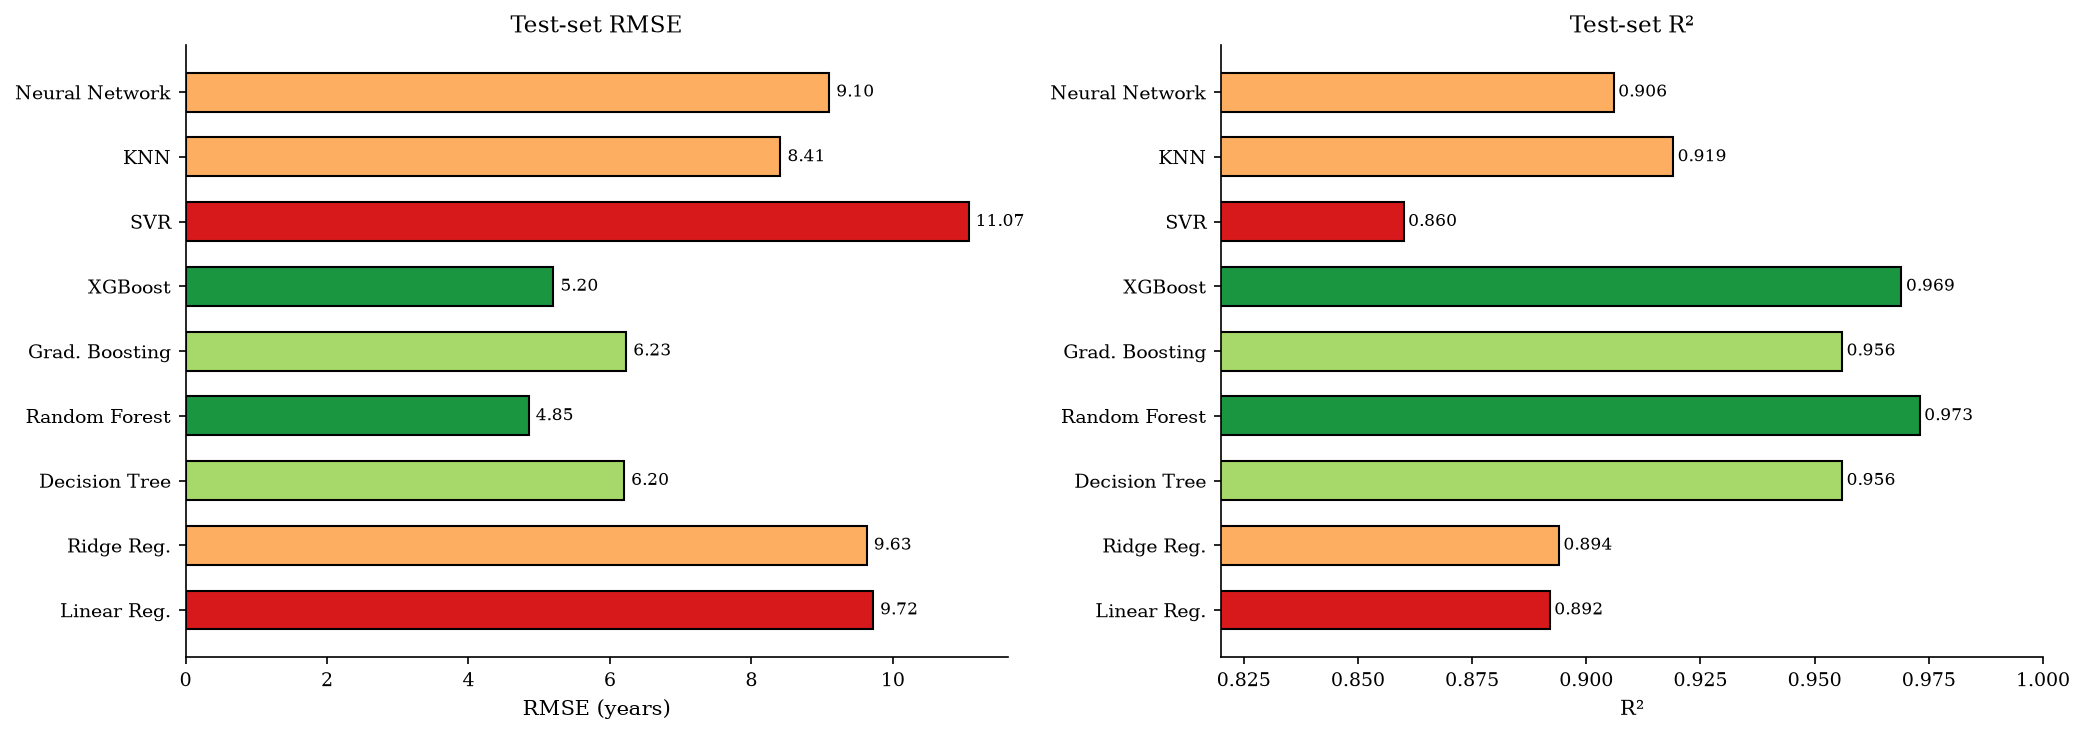
\includegraphics[width=\textwidth]{figures/fig_reg_comparison} 

}

\caption{\label{fig:reg-comp}Comparison of all nine regression models by test-set RMSE (left) and R\textsuperscript{2} (right). Colour indicates rank: green = top 2, light green = ranks 3--4, orange = ranks 5--7, red = bottom 2.}\label{fig:fig-reg-comp}
\end{figure}

Table \ref{tab:reg-cv} reports five-fold cross-validation results, which
broadly confirm the test-set ranking. The low standard deviations for
Random Forest (\(\pm 0.45\)) and Gradient Boosting (\(\pm 0.58\))
indicate stable generalisation. The Neural Network shows the highest CV
variance of any model (RMSE = 12.21 \(\pm\) 4.03), well above its single
test-set result of 9.10. This instability suggests the MLP's performance
depends on how the data are divided --- likely an interaction between
the default architecture and the uneven temporal distribution of
observations across folds.

\begin{longtable}[]{@{}lrr@{}}
\caption{\label{tab:reg-cv}Five-fold cross-validation results for
regression. CV RMSE is in years.}\tabularnewline
\toprule\noalign{}
Model & CV RMSE mean (yrs) & CV RMSE std \\
\midrule\noalign{}
\endfirsthead
\toprule\noalign{}
Model & CV RMSE mean (yrs) & CV RMSE std \\
\midrule\noalign{}
\endhead
\bottomrule\noalign{}
\endlastfoot
Linear Regression & 9.90 & 0.97 \\
Ridge Regression & 9.86 & 0.96 \\
Decision Tree & 7.64 & 0.59 \\
Random Forest & 5.24 & 0.45 \\
Gradient Boosting & 6.09 & 0.58 \\
XGBoost & 5.71 & 0.73 \\
SVR & 12.37 & 1.58 \\
KNN & 8.71 & 1.20 \\
Neural Network & 12.21 & 4.03 \\
\end{longtable}

Figure \ref{fig:reg-cv} displays the CV results with error bars, making
the instability of the linear models and the neural network visually
apparent.

\begin{figure}[htbp]

{\centering 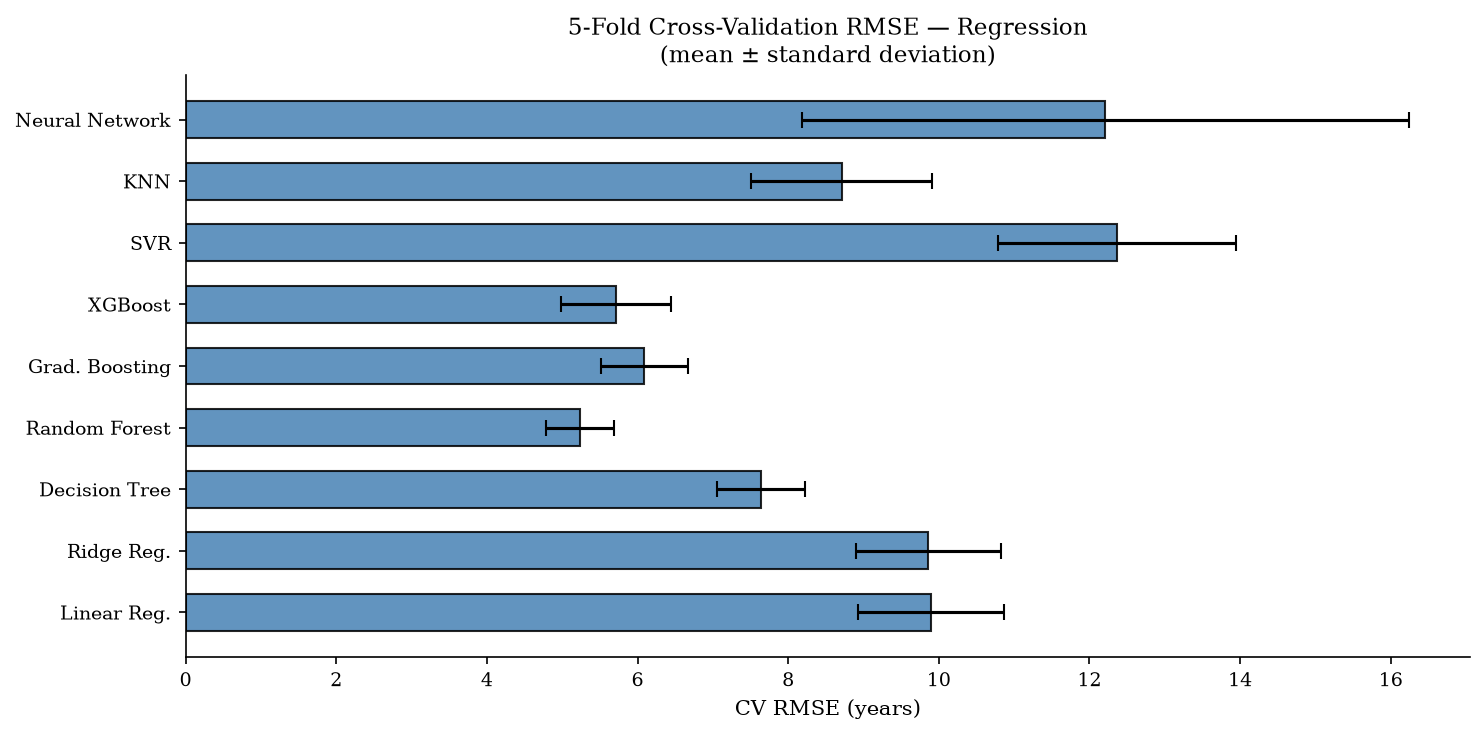
\includegraphics[width=\textwidth]{figures/fig_reg_cv} 

}

\caption{\label{fig:reg-cv}Five-fold cross-validation RMSE for all regression models (mean $\pm$ standard deviation).}\label{fig:fig-reg-cv}
\end{figure}

Figure \ref{fig:pred-actual} plots predicted against actual construction
year for the four best-performing models. The Random Forest and XGBoost
scatter plots show tight clustering around the perfect-prediction
diagonal, with no systematic over- or under-prediction across the year
range. The Ridge Regression plot shows a broader dispersion,
particularly for properties built before 1940, where the linear model's
inability to capture rare historical patterns is most apparent.

\begin{figure}[htbp]

{\centering 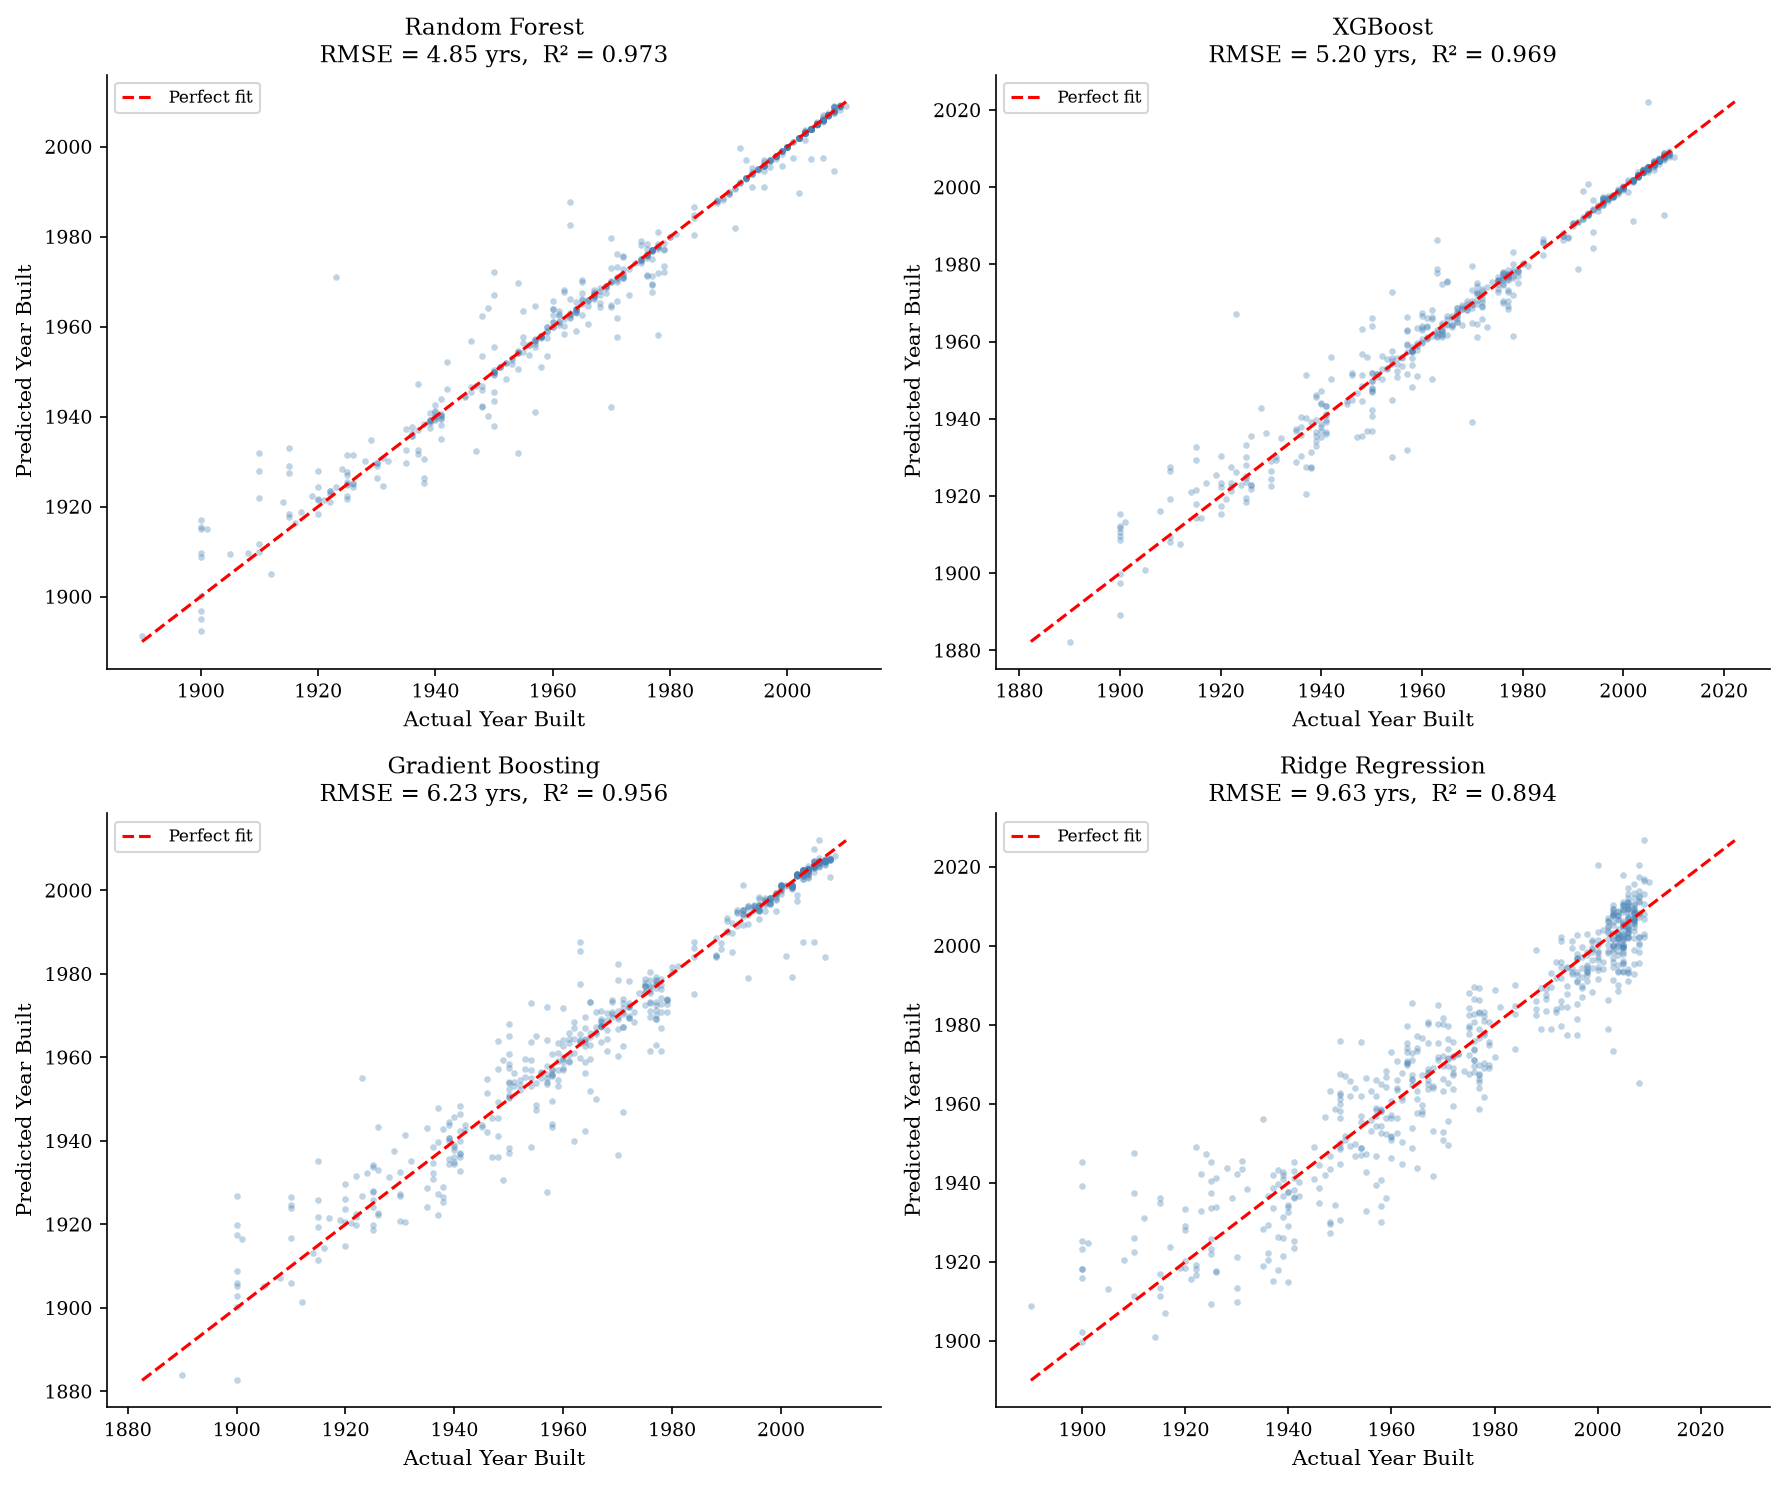
\includegraphics[width=\textwidth]{figures/fig_predicted_vs_actual} 

}

\caption{\label{fig:pred-actual}Predicted vs actual Year Built for the four best-performing regression models. The red dashed line marks perfect prediction. RMSE and R\textsuperscript{2} are reported in each panel title.}\label{fig:fig-pred-actual}
\end{figure}

Hyperparameter tuning produces divergent effects across the four models
searched. Table \ref{tab:reg-tuned} reports test-set performance after
tuning. Random Forest shows no improvement over its default
configuration (RMSE rises marginally from 4.85 to 4.87 years, within the
noise of a single train/test split), whereas Gradient Boosting and the
Support Vector Regressor both improve substantially (RMSE falling from
6.23 to 5.11 years, and from 11.07 to 8.56 years, respectively). XGBoost
improves moderately (from 5.20 to 4.90 years). Random Forest and XGBoost
retain the first and second positions held before tuning, but the
ranking narrows: all three tree-based ensembles now fall within 0.26
years of RMSE, while the tuned SVR remains clearly behind despite its
improvement. This pattern suggests Random Forest's default
hyperparameters were already well matched to this feature set, whereas
Gradient Boosting, XGBoost, and the SVR benefited from a targeted
search.

\begin{longtable}[]{@{}lrrr@{}}
\caption{\label{tab:reg-tuned}Regression results on the held-out test
set after hyperparameter tuning (n = 586). Only the four models selected
for tuning are shown; compare against the corresponding
default-hyperparameter rows in Table
\ref{tab:reg-results}.}\tabularnewline
\toprule\noalign{}
Model & MAE (yrs) & RMSE (yrs) & R\textsuperscript{2} \\
\midrule\noalign{}
\endfirsthead
\toprule\noalign{}
Model & MAE (yrs) & RMSE (yrs) & R\textsuperscript{2} \\
\midrule\noalign{}
\endhead
\bottomrule\noalign{}
\endlastfoot
Random Forest & 2.03 & 4.87 & 0.973 \\
Gradient Boosting & 2.53 & 5.11 & 0.970 \\
XGBoost & 2.50 & 4.90 & 0.973 \\
SVR & 4.93 & 8.56 & 0.917 \\
\end{longtable}

\subsection{Classification}\label{classification}

Table \ref{tab:clf-results} reports test-set performance across all
eight classifiers. XGBoost achieves the highest accuracy (91.5\%) and
macro F1 (0.833), followed closely by Gradient Boosting (91.3\%, F1 =
0.814). The gap between accuracy and macro F1 for most models reveals
the effect of class imbalance: models that correctly classify the
dominant Single-story class but struggle with Split-level properties
will show high accuracy but moderate F1.

\begin{longtable}[]{@{}lrrrr@{}}
\caption{\label{tab:clf-results}Classification results on the held-out
test set (n = 586). All metrics are macro-averaged across the four
typology classes.}\tabularnewline
\toprule\noalign{}
Model & Accuracy & Precision & Recall & F1 (macro) \\
\midrule\noalign{}
\endfirsthead
\toprule\noalign{}
Model & Accuracy & Precision & Recall & F1 (macro) \\
\midrule\noalign{}
\endhead
\bottomrule\noalign{}
\endlastfoot
Logistic Regression & 0.879 & 0.792 & 0.699 & 0.726 \\
Decision Tree & 0.850 & 0.736 & 0.754 & 0.744 \\
Random Forest & 0.899 & 0.897 & 0.728 & 0.763 \\
Gradient Boosting & 0.913 & 0.897 & 0.779 & 0.814 \\
XGBoost & 0.915 & 0.881 & 0.802 & 0.833 \\
SVC & 0.879 & 0.914 & 0.670 & 0.691 \\
KNN & 0.843 & 0.780 & 0.675 & 0.710 \\
Neural Network & 0.881 & 0.804 & 0.767 & 0.783 \\
\end{longtable}

\begin{figure}[htbp]

{\centering 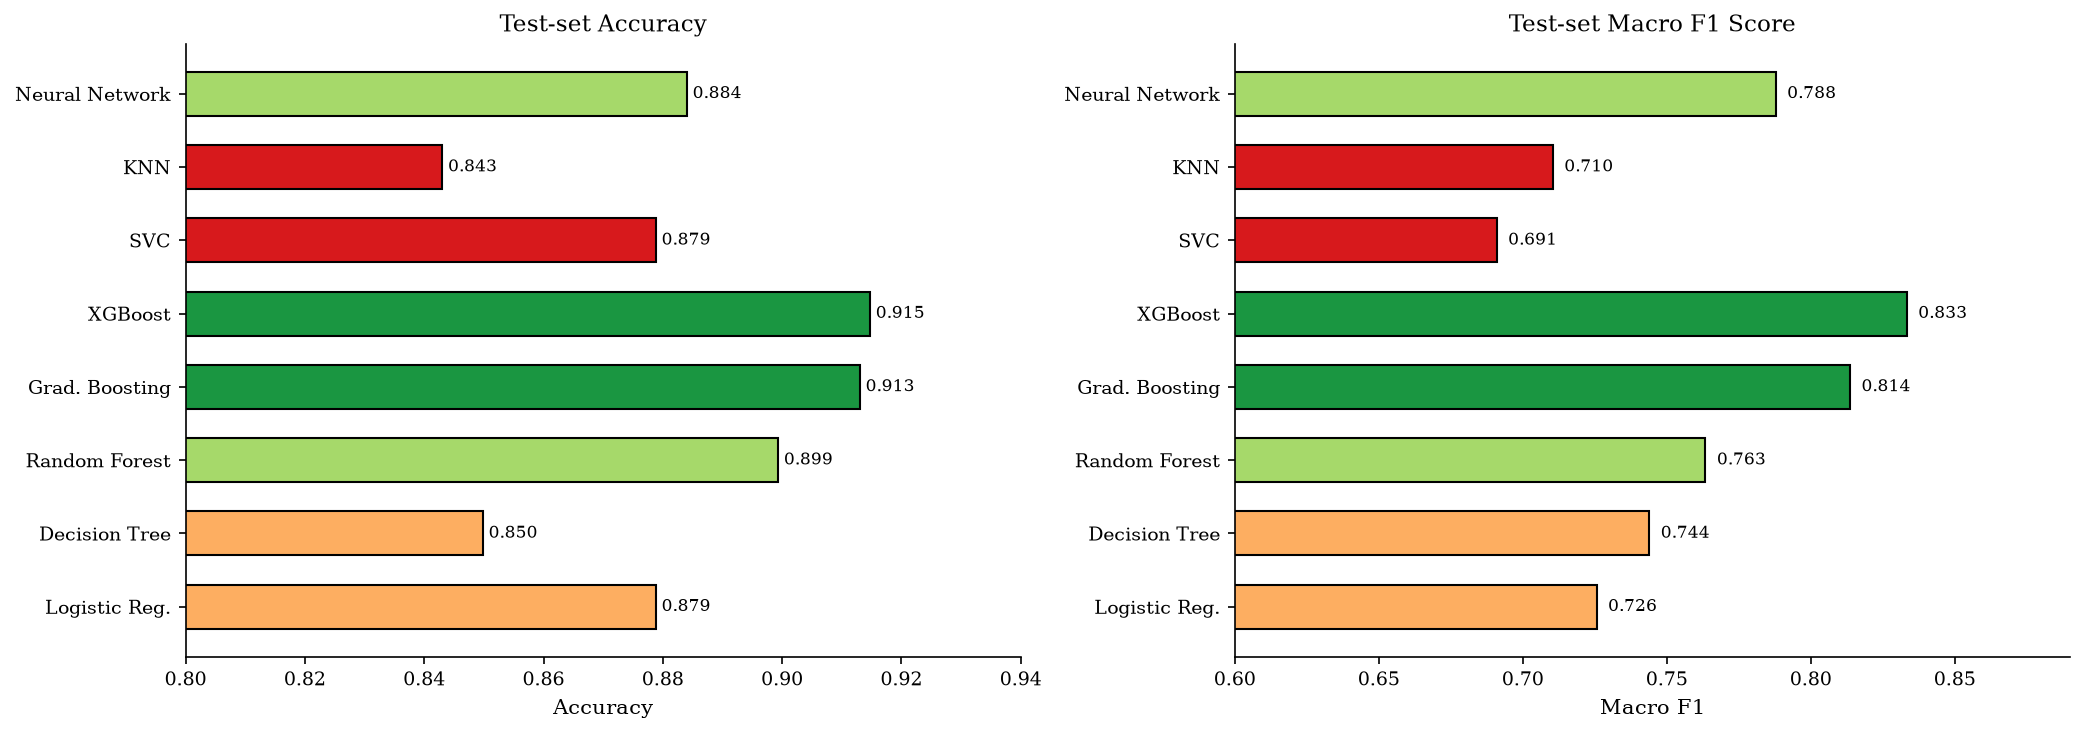
\includegraphics[width=\textwidth]{figures/fig_clf_comparison} 

}

\caption{\label{fig:clf-comp}Comparison of all eight classification models by test-set accuracy (left) and macro F1 score (right).}\label{fig:fig-clf-comp}
\end{figure}

Table \ref{tab:clf-cv} shows five-fold cross-validation results. The
ranking is consistent with the test set, and standard deviations are
small for most models. Gradient Boosting is notably stable (std =
0.006), while KNN shows the highest variability (std = 0.024),
reflecting sensitivity to local data density across folds.

\begin{longtable}[]{@{}lrr@{}}
\caption{\label{tab:clf-cv}Five-fold cross-validation accuracy for all
classification models.}\tabularnewline
\toprule\noalign{}
Model & CV Accuracy mean & CV Accuracy std \\
\midrule\noalign{}
\endfirsthead
\toprule\noalign{}
Model & CV Accuracy mean & CV Accuracy std \\
\midrule\noalign{}
\endhead
\bottomrule\noalign{}
\endlastfoot
Logistic Regression & 0.869 & 0.015 \\
Decision Tree & 0.852 & 0.018 \\
Random Forest & 0.904 & 0.011 \\
Gradient Boosting & 0.905 & 0.006 \\
XGBoost & 0.910 & 0.010 \\
SVC & 0.874 & 0.011 \\
KNN & 0.836 & 0.024 \\
Neural Network & 0.876 & 0.017 \\
\end{longtable}

\begin{figure}[htbp]

{\centering 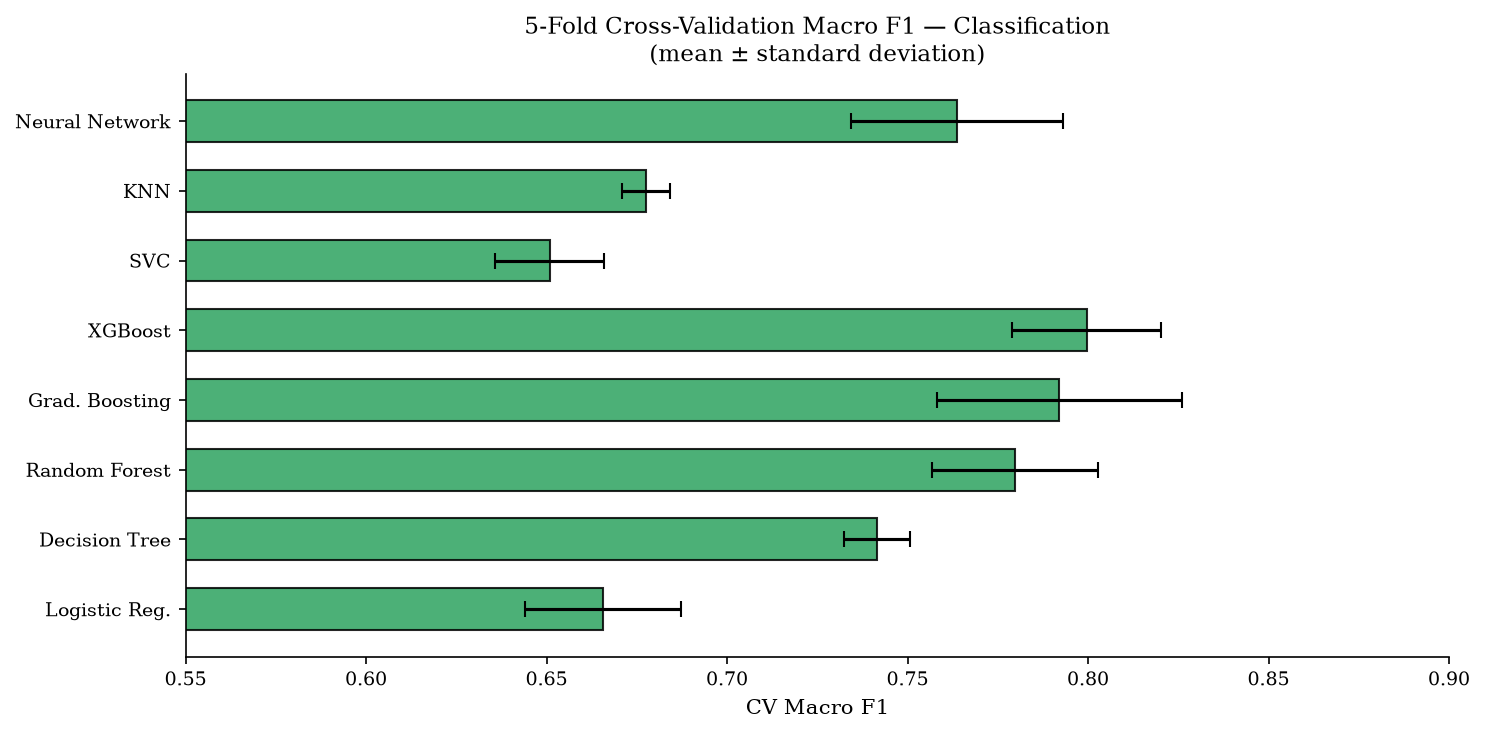
\includegraphics[width=\textwidth]{figures/fig_clf_cv} 

}

\caption{\label{fig:clf-cv}Five-fold cross-validation accuracy for all classification models (mean $\pm$ standard deviation).}\label{fig:fig-clf-cv}
\end{figure}

Table \ref{tab:clf-tuned} reports test-set performance after
hyperparameter tuning for the four classifiers selected. XGBoost
improves further to become the best-performing model overall (accuracy
91.8\%, macro F1 = 0.837, up from 0.833 untuned). The Support Vector
Classifier shows the largest gain from tuning of any model in either
task: macro F1 rises from 0.691 to 0.796, driven by a wider margin
parameter (\(C = 10\), against a default of \(C = 1\)) that allows the
decision boundary to extend further into minority-class regions.
Gradient Boosting's tuned macro F1 (0.811) is marginally below its
untuned value (0.814), a difference within the noise expected from
optimising on cross-validated F1 rather than the held-out test set
directly.

\begin{longtable}[]{@{}lrrrr@{}}
\caption{\label{tab:clf-tuned}Classification results on the held-out
test set after hyperparameter tuning (n = 586). Only the four models
selected for tuning are shown; compare against the corresponding
default-hyperparameter rows in Table
\ref{tab:clf-results}.}\tabularnewline
\toprule\noalign{}
Model & Accuracy & Precision & Recall & F1 (macro) \\
\midrule\noalign{}
\endfirsthead
\toprule\noalign{}
Model & Accuracy & Precision & Recall & F1 (macro) \\
\midrule\noalign{}
\endhead
\bottomrule\noalign{}
\endlastfoot
Random Forest & 0.899 & 0.893 & 0.735 & 0.770 \\
Gradient Boosting & 0.910 & 0.884 & 0.777 & 0.811 \\
XGBoost & 0.918 & 0.884 & 0.806 & 0.837 \\
SVC & 0.896 & 0.846 & 0.765 & 0.796 \\
\end{longtable}

Figure \ref{fig:confusion} shows the confusion matrix for the default
(pre-tuning) XGBoost classifier, which was the best-performing model at
that stage. The matrix reveals that Single-story and Multi-story
properties are classified with high accuracy, while 1.5-story properties
are occasionally misclassified as Multi-story and Split-level properties
show the highest error rate, primarily being predicted as Single-story
or Multi-story.

\begin{figure}[htbp]

{\centering 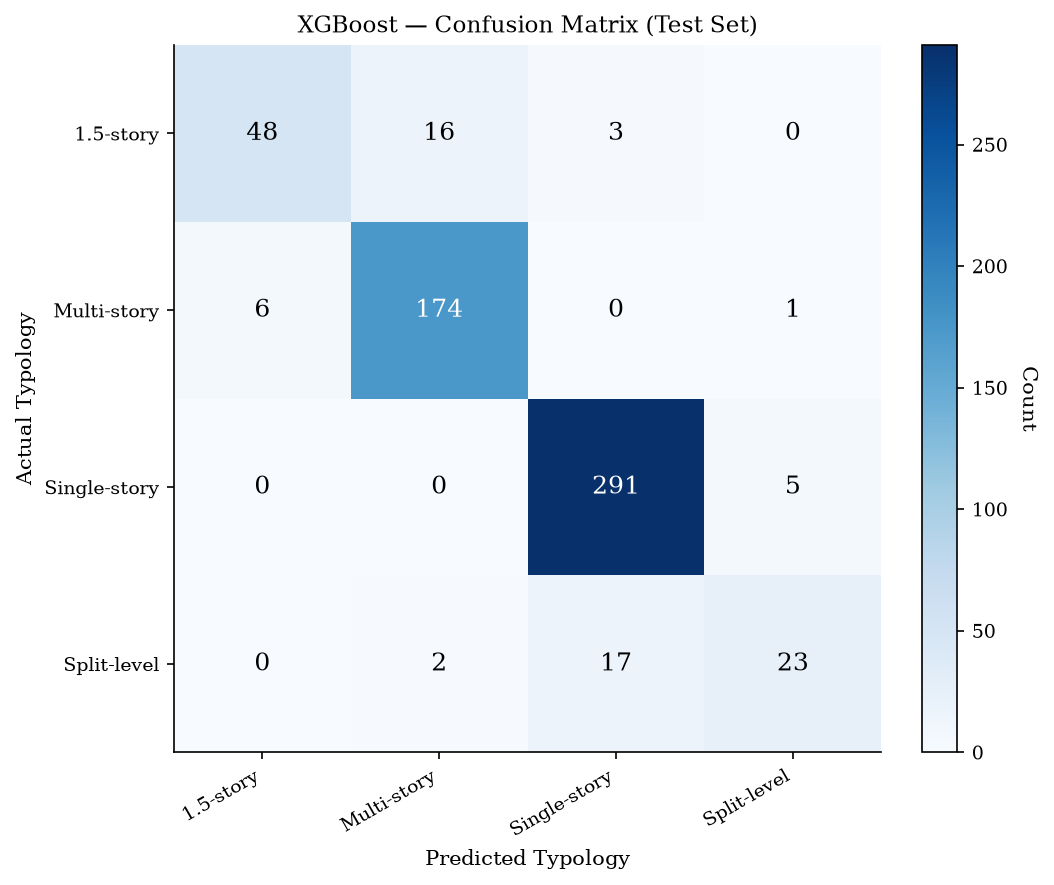
\includegraphics[width=0.7\textwidth]{figures/fig_confusion_matrix} 

}

\caption{\label{fig:confusion}Confusion matrix for the default (pre-tuning) XGBoost classifier on the held-out test set. Rows represent actual typology classes; columns represent predicted classes.}\label{fig:fig-confusion}
\end{figure}

\section{Discussion and Conclusion}\label{discussion-and-conclusion}

\subsection{Regression Task}\label{regression-task}

The strong performance of tree-based ensemble methods (Random Forest
\(R^2 = 0.973\), XGBoost \(R^2 = 0.969\)) confirms that a property's
physical attributes carry a chronological signal that machine learning
can recover with high accuracy. The clear advantage of non-linear
methods over linear baselines (\(R^2 \approx 0.89\)) is methodologically
informative: approximately 11\% of variance in construction year is
inaccessible to any linear combination of predictors, suggesting that
the relationship between physical attributes and construction era
involves threshold effects. This is consistent with the historical
structure of building practice --- materials and design standards did
not shift continuously but were subject to periodic regulatory and
technological step-changes, which decision boundaries in a tree can
represent directly.

The default SVR underperforms the other non-linear methods (RMSE =
11.07, \(R^2 = 0.860\)), indicating that its default radial basis
function kernel is poorly matched to this dataset's structure.
Hyperparameter tuning substantially narrows this gap (RMSE falls to
8.56, Table \ref{tab:reg-tuned}), confirming that the shortfall was
primarily a hyperparameter mismatch rather than a fundamental
unsuitability of margin-based methods for this task. Even tuned,
however, the SVR remains well behind the ensemble methods, indicating a
persistent structural disadvantage on this high-dimensional, mixed-type
feature set.

The neural network's cross-validation variance (RMSE = 12.21 \(\pm\)
4.03) is markedly higher than its single test-set result (RMSE = 9.10),
and higher than any tree-based model's CV variance. This divergence
suggests that the MLP's performance is fold-dependent rather than
robustly generalised. With 2,344 training observations and 150
post-encoding features, the default architecture likely lacks the
capacity to exploit deep interaction effects consistently, while the
uneven temporal distribution of observations across folds creates
varying learning conditions.

\subsection{Classification Task}\label{classification-task}

The classification results establish that architectural typology is
recoverable from geometric measurements with reasonable accuracy.
XGBoost is the strongest classifier both before tuning (91.5\% accuracy,
macro F1 = 0.833) and after (91.8\% accuracy, macro F1 = 0.837), making
it the best-performing model in either task after accounting for tuning.
The gap between accuracy and macro F1 highlights the effect of class
imbalance: the untuned SVC achieves 87.9\% accuracy but a macro F1 of
only 0.691, driven by low recall (0.670) for the minority classes. Its
high precision (0.914) indicates conservative decision boundaries ---
the model rarely ventures into minority-class territory, reserving those
predictions for high-confidence cases. Tuning corrects most of this
imbalance (macro F1 rises to 0.796, Table \ref{tab:clf-tuned}), which
confirms the untuned SVC's weakness was a hyperparameter mismatch rather
than an inherent limitation of margin-based classifiers on this feature
set. This behaviour is systematically visible in the confusion matrix
(Figure \ref{fig:confusion}): Split-level properties, which constitute
only 7.2\% of the dataset, are misclassified at a higher rate than any
other class.

The confusion between 1.5-story and Multi-story properties, and between
Split-level and Single-story properties, is architecturally
interpretable. Both 1.5-story and split-level forms occupy an
intermediate position in the floor-area space: a one-and-a-half story
home has a partial upper storey, and a split-level home has partial
floors at offset heights. The 30-feature geometric representation
captures aggregate measurements --- total area, room counts, basement
footprint --- but not the volumetric arrangement that distinguishes
these forms from a full two-story layout. This places a ceiling on
classification accuracy that is independent of model choice.

\subsection{Model Interpretability}\label{model-interpretability}

For the regression task, the two best models (Random Forest and XGBoost)
offer partial interpretability via feature importance. Both methods
identify Garage Year Built, Overall Quality, and Ground Living Area as
the most informative predictors --- a result that aligns with the
correlation analysis in Section \ref{exploratory-data-analysis}. For
applications where understanding which features drive a prediction is
important, XGBoost with SHAP values would provide the most operationally
useful explanations at the instance level.

The linear models (Linear Regression and Ridge) offer full
coefficient-level interpretability but at a substantial accuracy cost:
approximately 5 RMSE years relative to Random Forest. In settings where
interpretability is the primary constraint and approximate accuracy is
acceptable, Ridge Regression would be preferable. For most applications
of this type, the performance gap justifies the trade-off in favour of
Random Forest or XGBoost.

For classification, the Gradient Boosting and XGBoost classifiers offer
analogous interpretability properties to their regression counterparts.
The Decision Tree, though lower-performing, provides the most
transparent model: a single tree can be visualised and every prediction
traced to an explicit sequence of attribute thresholds. The similarity
between Decision Tree accuracy (85.0\%) and Logistic Regression accuracy
(87.9\%) suggests that non-linear boundaries alone do not account for
the performance advantage of ensemble methods; variance reduction
through aggregation is equally important.

\subsection{Limitations}\label{limitations}

Both tasks are evaluated on data from a single city over a four-year
period. The chronological signal exploited by the regression model
reflects construction norms specific to Ames, Iowa, and may not transfer
to other geographic or cultural contexts. The four-class typology
consolidation is one of several valid grouping choices; different
groupings would produce different class boundaries and potentially
different difficulty rankings for the classifiers.

Some geometric features retained in the classification feature set ---
such as garage size and basement finish level --- are themselves
correlated with construction era, which means the model may exploit an
indirect temporal signal rather than purely spatial information.
Disentangling these contributions would require a more controlled
feature selection procedure or a residualisation approach.

\subsection{Conclusion}\label{conclusion}

This study demonstrates that residential properties in the Ames Housing
Dataset carry two forms of latent architectural information ---
construction era and structural typology --- that machine learning can
recover with high accuracy. Random Forest achieves the strongest
regression performance (RMSE = 4.85 years, \(R^2 = 0.973\)) using its
default hyperparameters, and tuned XGBoost achieves the strongest
classification performance (accuracy = 91.8\%, macro F1 = 0.837). In
both tasks, tree-based ensemble methods --- bagged (Random Forest) or
boosted (Gradient Boosting, XGBoost) --- consistently outperform linear,
kernel-based, and instance-based alternatives. Cross-validation confirms
that these results are stable and not artefacts of a favourable
train/test split.

From a methodological standpoint, the study illustrates three recurring
considerations in tabular machine learning: the value of leakage-safe
preprocessing pipelines, the importance of selecting evaluation metrics
that account for class imbalance, and the trade-off between predictive
accuracy and model interpretability. When the accuracy margin justifies
it, ensemble methods provide an effective combination of strong
generalisation and partial explainability through feature importance ---
a balance that makes them well suited to structured prediction tasks on
housing data.
\renewcommand*{\mkbibnamefamily}[1]{\textbf{#1}}
\renewcommand*{\mkbibnamegiven}[1]{\textbf{#1}}
\renewcommand*{\mkbibnameprefix}[1]{\textbf{#1}}
\renewcommand*{\mkbibnamesuffix}[1]{\textbf{#1}}
\printbibliography[title=References]

\newpage
\textbf{Eidesstattliche Versicherung}

\bigskip

Ich versichere an Eides statt durch meine Unterschrift, dass ich die vorstehende Arbeit selbständig und ohne fremde Hilfe angefertigt und alle Stellen, die ich wörtlich oder annähernd wörtlich aus Veröffentlichungen entnommen habe, als solche kenntlich gemacht habe, mich auch keiner anderen als der angegebenen Literatur oder sonstiger Hilfsmittel bedient habe. Die Arbeit hat in dieser oder ähnlicher Form noch keiner anderen Prüfungsbehörde vorgelegen.

\vspace{1cm}
\rule{0pt}{2\baselineskip} %
\par\noindent\makebox[2.25in]{\indent Essen, den \hrulefill} \hfill\makebox[2.25in]{\hrulefill}%
\par\noindent\makebox[2.25in][l]{} \hfill\makebox[2.25in][c]{Rezaul
Hoque, Sarah Al-Talal}%

\end{document}
